\hypertarget{sec-pipelines-nonseq}{%
\chapter{Non-sequential Pipelines and Tuning}\label{sec-pipelines-nonseq}}

\vspace{-15mm}\addtocontents{toc}{\textit{Martin Binder, Florian Pfisterer, Marc Becker and Marvin N. Wright}}

\textbf{Martin Binder} \newline  \emph{Ludwig-Maximilians-Universität
München, and Munich Center for Machine Learning (MCML)}

\textbf{Florian Pfisterer} \newline 
\emph{Ludwig-Maximilians-Universität München}

\textbf{Marc Becker} \newline  \emph{Ludwig-Maximilians-Universität
München, and Munich Center for Machine Learning (MCML)}

\textbf{Marvin N. Wright} \newline  \emph{Leibniz Institute for
Prevention Research and Epidemiology -- BIPS, and University of Bremen,
and University of Copenhagen} \newline \newline 

In Chapter~\ref{sec-pipelines} we looked at simple sequential pipelines
that can be built using the
\href{https://mlr3pipelines.mlr-org.com/reference/Graph.html}{\texttt{Graph}}
class and a few
\href{https://mlr3pipelines.mlr-org.com/reference/PipeOp.html}{\texttt{PipeOp}}
objects. In this chapter, we will take this further and look at
non-sequential pipelines that can perform more complex operations. We
will then look at tuning pipelines by combining methods in
\href{https://mlr3tuning.mlr-org.com}{\texttt{mlr3tuning}}\index{\texttt{mlr3tuning}}
and
\href{https://mlr3pipelines.mlr-org.com}{\texttt{mlr3pipelines}}\index{\texttt{mlr3pipelines}}
and will consider some concrete examples using multi-fidelity tuning
(Section~\ref{sec-hyperband}) and feature selection
(Chapter~\ref{sec-feature-selection}).

We saw the power of the
\texttt{\%\textgreater{}\textgreater{}\%}-operator in
Chapter~\ref{sec-pipelines} to assemble graphs from combinations of
multiple \texttt{PipeOp}s and \texttt{Learner}s. Given a single
\texttt{PipeOp} or
\href{https://mlr3.mlr-org.com/reference/Learner.html}{\texttt{Learner}},
the \texttt{\%\textgreater{}\textgreater{}\%}-operator will arrange
these objects into a linear \texttt{Graph} with each \texttt{PipeOp}
acting in sequence. However, by using the
\href{https://mlr3pipelines.mlr-org.com/reference/gunion.html}{\texttt{gunion()}}
function, we can instead combine multiple \texttt{PipeOp}s,
\texttt{Graph}s, or a mixture of both, into a parallel \texttt{Graph}.

In the following example, we create a \texttt{Graph} that centers its
inputs (\texttt{po("scale")}) and then copies the centered data to two
parallel streams: one replaces the data with columns that indicate
whether data is missing (\texttt{po("missind")}), and the other imputes
missing data using the median (\texttt{po("imputemedian")}), which we
will return to in Section~\ref{sec-preprocessing-missing}. The outputs
of both streams are then combined into a single dataset using
\texttt{po("featureunion")}.

\begin{Shaded}
\begin{Highlighting}[]
\FunctionTok{library}\NormalTok{(mlr3pipelines)}

\NormalTok{graph }\OtherTok{=} \FunctionTok{po}\NormalTok{(}\StringTok{"scale"}\NormalTok{, }\AttributeTok{center =} \ConstantTok{TRUE}\NormalTok{, }\AttributeTok{scale =} \ConstantTok{FALSE}\NormalTok{) }\SpecialCharTok{\%\textgreater{}\textgreater{}\%}
  \FunctionTok{gunion}\NormalTok{(}\FunctionTok{list}\NormalTok{(}
    \FunctionTok{po}\NormalTok{(}\StringTok{"missind"}\NormalTok{),}
    \FunctionTok{po}\NormalTok{(}\StringTok{"imputemedian"}\NormalTok{)}
\NormalTok{  )) }\SpecialCharTok{\%\textgreater{}\textgreater{}\%}
  \FunctionTok{po}\NormalTok{(}\StringTok{"featureunion"}\NormalTok{)}

\NormalTok{graph}\SpecialCharTok{$}\FunctionTok{plot}\NormalTok{(}\AttributeTok{horizontal =} \ConstantTok{TRUE}\NormalTok{)}
\end{Highlighting}
\end{Shaded}

\begin{figure}

{\centering \includegraphics[width=1\textwidth,height=\textheight]{chapters/chapter8/non-sequential_pipelines_and_tuning_files/figure-pdf/fig-pipelines-parallel-plot-1.png}

}

\caption{\label{fig-pipelines-parallel-plot}Simple parallel pipeline
plot showing a common data source being scaled then the same data being
passed to two \texttt{PipeOp}s in parallel whose outputs are combined
and returned to the user.}

\end{figure}

When applied to the first three rows of the \texttt{"pima"} task we can
see how this imputes missing data and adds a column indicating where
values were missing.

\begin{Shaded}
\begin{Highlighting}[]
\NormalTok{tsk\_pima\_head }\OtherTok{=} \FunctionTok{tsk}\NormalTok{(}\StringTok{"pima"}\NormalTok{)}\SpecialCharTok{$}\FunctionTok{filter}\NormalTok{(}\DecValTok{1}\SpecialCharTok{:}\DecValTok{3}\NormalTok{)}
\NormalTok{tsk\_pima\_head}\SpecialCharTok{$}\FunctionTok{data}\NormalTok{(}\AttributeTok{cols =} \FunctionTok{c}\NormalTok{(}\StringTok{"diabetes"}\NormalTok{, }\StringTok{"insulin"}\NormalTok{, }\StringTok{"triceps"}\NormalTok{))}
\end{Highlighting}
\end{Shaded}

\begin{verbatim}
   diabetes insulin triceps
1:      pos      NA      35
2:      neg      NA      29
3:      pos      NA      NA
\end{verbatim}

\begin{Shaded}
\begin{Highlighting}[]
\NormalTok{result }\OtherTok{=}\NormalTok{ graph}\SpecialCharTok{$}\FunctionTok{train}\NormalTok{(tsk\_pima\_head)[[}\DecValTok{1}\NormalTok{]]}
\NormalTok{result}\SpecialCharTok{$}\FunctionTok{data}\NormalTok{(}\AttributeTok{cols =} \FunctionTok{c}\NormalTok{(}\StringTok{"diabetes"}\NormalTok{, }\StringTok{"insulin"}\NormalTok{, }\StringTok{"missing\_insulin"}\NormalTok{, }\StringTok{"triceps"}\NormalTok{,}
  \StringTok{"missing\_triceps"}\NormalTok{))}
\end{Highlighting}
\end{Shaded}

\begin{verbatim}
   diabetes insulin missing_insulin triceps missing_triceps
1:      pos       0         missing       3         present
2:      neg       0         missing      -3         present
3:      pos       0         missing       0         missing
\end{verbatim}

\hypertarget{selectors-and-parallel-pipelines}{%
\section{Selectors and Parallel
Pipelines}\label{selectors-and-parallel-pipelines}}

It is common in
\href{https://mlr3pipelines.mlr-org.com/reference/Graph.html}{\texttt{Graph}}s
for an operation to be applied to a subset of features. In
\texttt{mlr3pipelines} this can be achieved in two ways
(Figure~\ref{fig-pipelines-select-affect}): either by passing the column
subset to the \texttt{affect\_columns} hyperparameter of a
\href{https://mlr3pipelines.mlr-org.com/reference/PipeOp.html}{\texttt{PipeOp}}
(assuming it has that hyperparameter), which controls which columns
should be affected by the \texttt{PipeOp}; or, one can use the
\href{https://mlr3pipelines.mlr-org.com/reference/mlr_pipeops_select.html}{\texttt{PipeOpSelect}}\index{\texttt{PipeOpSelect}}
operator to create operations in parallel on specified feature subsets,
and then unite the result using
\href{https://mlr3pipelines.mlr-org.com/reference/mlr_pipeops_featureunion.html}{\texttt{PipeOpFeatureUnion}}.

\begin{figure}

\begin{minipage}[t]{\linewidth}

{\centering 

\raisebox{-\height}{

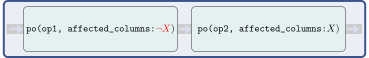
\includegraphics{chapters/chapter8/Figures/mlr3book_figures-28.png}

}

}

\subcaption{\label{fig-pipelines-select-affect-1}The
\texttt{affect\_columns} hyperparameter can be used to restrict
operations to a subset of features. When used, pipelines may still be
run in sequence.}
\end{minipage}%
\newline
\begin{minipage}[t]{\linewidth}

{\centering 

\raisebox{-\height}{

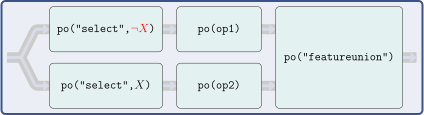
\includegraphics{chapters/chapter8/Figures/mlr3book_figures-29.png}

}

}

\subcaption{\label{fig-pipelines-select-affect-2}Operating on subsets of
tasks using concurrent paths by first splitting the inputs with
\texttt{po("select")} and then combining outputs with
\texttt{po("featureunion")}.}
\end{minipage}%

\caption{\label{fig-pipelines-select-affect}Two methods of setting up
\texttt{PipeOp}s (\texttt{po(op1)} and \texttt{po(op2)}) that operate on
complementary features (X and ¬X) of an input task.}

\end{figure}

Both methods make use of
\href{https://mlr3pipelines.mlr-org.com/reference/Selector.html}{\texttt{Selector}}\index{\texttt{Selector}}{\marginnote{\begin{footnotesize}\texttt{Selector}\end{footnotesize}}}-functions.
These are helper functions that indicate to a \texttt{PipeOp} which
features it should apply to. \texttt{Selectors} may match column names
by regular expressions
(\href{https://mlr3pipelines.mlr-org.com/reference/Selector.html}{\texttt{selector\_grep()}}),
or by column type
(\href{https://mlr3pipelines.mlr-org.com/reference/Selector.html}{\texttt{selector\_type()}}).
\texttt{Selectors} can also be used to join variables
(\href{https://mlr3pipelines.mlr-org.com/reference/Selector.html}{\texttt{selector\_union()}}),
return their set difference
(\href{https://mlr3pipelines.mlr-org.com/reference/Selector.html}{\texttt{selector\_setdiff()}}),
or select the complement of features from another \texttt{Selector}
(\href{https://mlr3pipelines.mlr-org.com/reference/Selector.html}{\texttt{selector\_invert()}}).

For example, in Section~\ref{sec-pipelines-pipeops} we applied PCA to
the bill length and depth of penguins from
\texttt{tsk("penguins\_simple")} by first selecting these columns using
the \texttt{Task} method \texttt{\$select()} and then applying the
\texttt{PipeOp}. We can now do this more simply with
\texttt{selector\_grep}, and could go on to use
\texttt{selector\_invert} to apply some other \texttt{PipeOp} to other
features, below we use \texttt{po("scale")} and make use of the
\texttt{affect\_columns} hyperparameter:

\begin{Shaded}
\begin{Highlighting}[]
\NormalTok{sel\_bill }\OtherTok{=} \FunctionTok{selector\_grep}\NormalTok{(}\StringTok{"\^{}bill"}\NormalTok{)}
\NormalTok{sel\_not\_bill }\OtherTok{=} \FunctionTok{selector\_invert}\NormalTok{(sel\_bill)}

\NormalTok{graph }\OtherTok{=} \FunctionTok{po}\NormalTok{(}\StringTok{"scale"}\NormalTok{, }\AttributeTok{affect\_columns =}\NormalTok{ sel\_not\_bill) }\SpecialCharTok{\%\textgreater{}\textgreater{}\%}
  \FunctionTok{po}\NormalTok{(}\StringTok{"pca"}\NormalTok{, }\AttributeTok{affect\_columns =}\NormalTok{ sel\_bill)}

\NormalTok{result }\OtherTok{=}\NormalTok{ graph}\SpecialCharTok{$}\FunctionTok{train}\NormalTok{(}\FunctionTok{tsk}\NormalTok{(}\StringTok{"penguins\_simple"}\NormalTok{))}
\NormalTok{result[[}\DecValTok{1}\NormalTok{]]}\SpecialCharTok{$}\FunctionTok{data}\NormalTok{()[}\DecValTok{1}\SpecialCharTok{:}\DecValTok{3}\NormalTok{, }\DecValTok{1}\SpecialCharTok{:}\DecValTok{5}\NormalTok{]}
\end{Highlighting}
\end{Shaded}

\begin{verbatim}
   species    PC1     PC2 body_mass flipper_length
1:  Adelie -5.015  1.0717   -0.5676        -1.4246
2:  Adelie -4.495 -0.1853   -0.5055        -1.0679
3:  Adelie -3.755  0.4868   -1.1886        -0.4257
\end{verbatim}

The biggest advantage of this method is that it creates a very simple,
sequential \texttt{Graph}. However, one disadvantage of the
\texttt{affect\_columns} method is that it is relatively easy to have
unexpected results if the ordering of \texttt{PipeOp}s is mixed up. For
example, if we had reversed the order of \texttt{po("pca")} and
\texttt{po("scale")} above then we would have first created columns
\texttt{"PC1"} and \texttt{"PC2"} and then erroneously scaled these,
since their names do not start with ``bill'' and they are therefore
matched by \texttt{sel\_not\_bill}. Creating parallel paths with
\texttt{po("select")} can help mitigate such errors by selecting
features given by the \texttt{Selector} and creating independent data
processing streams with the given feature subset. Below we pass the
parallel pipelines to
\href{https://mlr3pipelines.mlr-org.com/reference/gunion.html}{\texttt{gunion()}}
as a \texttt{list} to ensure they receive the same input, and then
combine the outputs with \texttt{po("featureunion")}.

\begin{Shaded}
\begin{Highlighting}[]
\NormalTok{po\_select\_bill }\OtherTok{=} \FunctionTok{po}\NormalTok{(}\StringTok{"select"}\NormalTok{, }\AttributeTok{id =} \StringTok{"s\_bill"}\NormalTok{, }\AttributeTok{selector =}\NormalTok{ sel\_bill)}
\NormalTok{po\_select\_not\_bill }\OtherTok{=} \FunctionTok{po}\NormalTok{(}\StringTok{"select"}\NormalTok{, }\AttributeTok{id =} \StringTok{"s\_notbill"}\NormalTok{,}
  \AttributeTok{selector =}\NormalTok{ sel\_not\_bill)}

\NormalTok{path\_pca }\OtherTok{=}\NormalTok{  po\_select\_bill }\SpecialCharTok{\%\textgreater{}\textgreater{}\%} \FunctionTok{po}\NormalTok{(}\StringTok{"pca"}\NormalTok{)}
\NormalTok{path\_scale }\OtherTok{=}\NormalTok{ po\_select\_not\_bill }\SpecialCharTok{\%\textgreater{}\textgreater{}\%} \FunctionTok{po}\NormalTok{(}\StringTok{"scale"}\NormalTok{)}

\NormalTok{graph }\OtherTok{=} \FunctionTok{gunion}\NormalTok{(}\FunctionTok{list}\NormalTok{(path\_pca, path\_scale)) }\SpecialCharTok{\%\textgreater{}\textgreater{}\%} \FunctionTok{po}\NormalTok{(}\StringTok{"featureunion"}\NormalTok{)}
\NormalTok{graph}\SpecialCharTok{$}\FunctionTok{plot}\NormalTok{(}\AttributeTok{horizontal =} \ConstantTok{TRUE}\NormalTok{)}
\end{Highlighting}
\end{Shaded}

\begin{figure}

{\centering \includegraphics[width=1\textwidth,height=\textheight]{chapters/chapter8/non-sequential_pipelines_and_tuning_files/figure-pdf/fig-pipelines-pcascale-1.png}

}

\caption{\label{fig-pipelines-pcascale}Visualization of a \texttt{Graph}
where features are split into two paths, one with PCA and one with
scaling, then combined and returned.}

\end{figure}

The \texttt{po("select")} method also has the significant advantage that
it allows the same set of features to be used in multiple operations
simultaneously, or to both transform features and keep their
untransformed versions (by using \texttt{po("nop")} in one path).
\href{https://mlr3pipelines.mlr-org.com/reference/mlr_pipeops_nop.html}{\texttt{PipeOpNOP}}
performs no operation on its inputs and is thus useful when you only
want to perform a transformation on a subset of features and leave the
others untouched:

\begin{Shaded}
\begin{Highlighting}[]
\NormalTok{graph }\OtherTok{=} \FunctionTok{gunion}\NormalTok{(}\FunctionTok{list}\NormalTok{(}
\NormalTok{  po\_select\_bill }\SpecialCharTok{\%\textgreater{}\textgreater{}\%} \FunctionTok{po}\NormalTok{(}\StringTok{"scale"}\NormalTok{),}
\NormalTok{  po\_select\_not\_bill }\SpecialCharTok{\%\textgreater{}\textgreater{}\%} \FunctionTok{po}\NormalTok{(}\StringTok{"nop"}\NormalTok{)}
\NormalTok{)) }\SpecialCharTok{\%\textgreater{}\textgreater{}\%} \FunctionTok{po}\NormalTok{(}\StringTok{"featureunion"}\NormalTok{)}
\NormalTok{graph}\SpecialCharTok{$}\FunctionTok{plot}\NormalTok{(}\AttributeTok{horizontal =} \ConstantTok{TRUE}\NormalTok{)}
\end{Highlighting}
\end{Shaded}

\begin{figure}

{\centering \includegraphics[width=1\textwidth,height=\textheight]{chapters/chapter8/non-sequential_pipelines_and_tuning_files/figure-pdf/fig-pipelines-selectnop-1.png}

}

\caption{\label{fig-pipelines-selectnop}Visualization of our
\texttt{Graph} where features are split into two paths, features that
start with `bill' are scaled and the rest are untransformed.}

\end{figure}

\begin{Shaded}
\begin{Highlighting}[]
\NormalTok{graph}\SpecialCharTok{$}\FunctionTok{train}\NormalTok{(}\FunctionTok{tsk}\NormalTok{(}\StringTok{"penguins\_simple"}\NormalTok{))[[}\DecValTok{1}\NormalTok{]]}\SpecialCharTok{$}\FunctionTok{data}\NormalTok{()[}\DecValTok{1}\SpecialCharTok{:}\DecValTok{3}\NormalTok{, }\DecValTok{1}\SpecialCharTok{:}\DecValTok{5}\NormalTok{]}
\end{Highlighting}
\end{Shaded}

\begin{verbatim}
   species bill_depth bill_length body_mass flipper_length
1:  Adelie     0.7796     -0.8947      3750            181
2:  Adelie     0.1194     -0.8216      3800            186
3:  Adelie     0.4241     -0.6753      3250            195
\end{verbatim}

\hypertarget{sec-pipelines-ppl}{%
\section{Common Patterns and ppl()}\label{sec-pipelines-ppl}}

Now you have the tools to create sequential and non-sequential
pipelines, you can create an infinite number of transformations on
\href{https://mlr3.mlr-org.com/reference/Task.html}{\texttt{Task}},
\href{https://mlr3.mlr-org.com/reference/Learner.html}{\texttt{Learner}},
and
\href{https://mlr3.mlr-org.com/reference/Prediction.html}{\texttt{Prediction}}
objects. In Section~\ref{sec-pipelines-bagging} and
Section~\ref{sec-pipelines-stack} we will work through two examples to
demonstrate how you can make complex and powerful graphs using the
methods and classes we have already looked at. However, many common
problems in ML can be well solved by the same pipelines, and so to make
your life easier we have implemented and saved these pipelines in the
\href{https://mlr3pipelines.mlr-org.com/reference/mlr_graphs.html}{\texttt{mlr\_graphs}}\index{\texttt{mlr\_graphs}}
dictionary; pipelines in the dictionary can be accessed with the
\href{https://mlr3pipelines.mlr-org.com/reference/ppl.html}{\texttt{ppl()}}\index{\texttt{ppl()}}{\marginnote{\begin{footnotesize}\texttt{ppl()}\end{footnotesize}}}
sugar function.

At the time of writing, this dictionary includes seven
\href{https://mlr3pipelines.mlr-org.com/reference/Graph.html}{\texttt{Graph}}s
(required arguments included below):

\begin{itemize}
\tightlist
\item
  \texttt{ppl("bagging",\ graph)}: In \texttt{mlr3pipelines},
  bagging\index{bagging} is the process of running a \texttt{graph}
  multiple times on different data samples and then averaging the
  results. This is discussed in detail in
  Section~\ref{sec-pipelines-bagging}.
\item
  \texttt{ppl("branch",\ graphs)}: Uses
  \href{https://mlr3pipelines.mlr-org.com/reference/mlr_pipeops_branch.html}{\texttt{PipeOpBranch}}
  to create different path branches from the given \texttt{graphs} where
  only one branch is evaluated. This is returned to in more detail in
  Section~\ref{sec-pipelines-branch}.
\item
  \texttt{ppl("greplicate",\ graph,\ n)}: Create a \texttt{Graph} that
  replicates \texttt{graph} (which can also be a single \texttt{PipeOp})
  \texttt{n} times. The pipeline avoids ID clashes by adding a suffix to
  each \texttt{PipeOp}, we will see this pipeline in use in
  Section~\ref{sec-pipelines-bagging}.
\item
  \texttt{ppl("ovr",\ graph)}: One-versus-rest
  classification\index{one-versus-rest classification} for converting
  multiclass classification\index{classification!multiclass} tasks into
  several binary classification tasks with one task for each class in
  the original. These tasks are then evaluated by the given
  \texttt{graph}, which should be a learner (or a pipeline containing a
  learner that emits a prediction). The predictions made on the binary
  tasks are combined into the multiclass prediction needed for the
  original task.
\item
  \texttt{ppl("robustify")}: Performs common preprocessing steps to make
  any \texttt{Task} compatible with a given \texttt{Learner}. This
  pipeline is demonstrated in Section~\ref{sec-prepro-robustify}.
\item
  \texttt{ppl("stacking",\ base\_learners,\ super\_learner)}:
  Stacking\index{stacking}, returned to in detail in
  Section~\ref{sec-pipelines-stack}, is the process of using predictions
  from one or more models (\texttt{base\_learners}) as features in a
  subsequent model (\texttt{super\_learner})
\item
  \texttt{ppl("targettrafo",\ graph)}: Create a \texttt{Graph} that
  transforms the prediction target of a task and ensures that any
  transformations applied during training (using the function passed to
  the \texttt{targetmutate.trafo} hyperparameter) are inverted in the
  resulting predictions (using the function passed to the
  \texttt{targetmutate.inverter} hyperparameter); an example is given in
  Section~\ref{sec-prepro-scale}.
\end{itemize}

\hypertarget{practical-pipelines-by-example}{%
\section{Practical Pipelines by
Example}\label{practical-pipelines-by-example}}

In this section, we will put pipelines into practice by demonstrating
how to turn weak learners into powerful machine learning models using
bagging\index{bagging} and stacking\index{stacking}.

\hypertarget{sec-pipelines-bagging}{%
\subsection{Bagging with ``greplicate'' and
``subsample''}\label{sec-pipelines-bagging}}

The basic idea of bagging\index{bagging} (from \textbf{b}ootstrapp
\textbf{agg}regat\textbf{ing}), introduced by Breiman (1996), is to
aggregate multiple predictors into a single, more powerful predictor
(Figure~\ref{fig-pipelines-bagging}). Predictions are usually aggregated
by the arithmetic mean for regression tasks or majority vote for
classification. The underlying intuition behind bagging is that
averaging a set of unstable and diverse (i.e., only weakly correlated)
predictors can reduce the variance of the overall prediction. Each
learner is trained on a different random sample of the original data.

Although we have already seen that a pre-constructed bagging pipeline is
available with \texttt{ppl("bagging")}, in this section we will build
our own pipeline from scratch to showcase how to construct a complex
\href{https://mlr3pipelines.mlr-org.com/reference/Graph.html}{\texttt{Graph}},
which will look something like Figure~\ref{fig-pipelines-bagging}.

\begin{figure}

{\centering 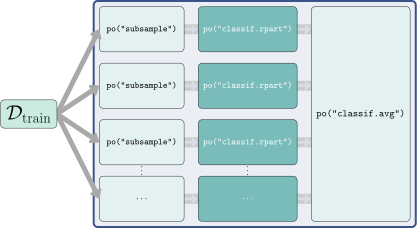
\includegraphics[width=0.7\textwidth,height=\textheight]{chapters/chapter8/Figures/mlr3book_figures-26.png}

}

\caption{\label{fig-pipelines-bagging}Graph that performs Bagging by
independently subsampling data and fitting individual decision tree
learners. The resulting predictions are aggregated by a majority vote
\texttt{PipeOp}.}

\end{figure}

To begin, we use \texttt{po("subsample")} to sample a fraction of the
data (here 70\%), which is then passed to a classification tree (note by
default \texttt{po("subsample")} samples without replacement).

\begin{Shaded}
\begin{Highlighting}[]
\NormalTok{gr\_single\_pred }\OtherTok{=} \FunctionTok{po}\NormalTok{(}\StringTok{"subsample"}\NormalTok{, }\AttributeTok{frac =} \FloatTok{0.7}\NormalTok{) }\SpecialCharTok{\%\textgreater{}\textgreater{}\%} \FunctionTok{lrn}\NormalTok{(}\StringTok{"classif.rpart"}\NormalTok{)}
\end{Highlighting}
\end{Shaded}

Next, we use \texttt{ppl("greplicate")} to copy the graph,
\texttt{gr\_single\_pred}, 10 times (\texttt{n\ =\ 10}) and finally
\texttt{po("classifavg")} to take the majority vote of all predictions,
note that we pass \texttt{innum\ =\ 10} to \texttt{"classifavg"} to tell
the
\href{https://mlr3pipelines.mlr-org.com/reference/PipeOp.html}{\texttt{PipeOp}}
to expect 10 inputs.

\begin{Shaded}
\begin{Highlighting}[]
\NormalTok{gr\_pred\_set }\OtherTok{=} \FunctionTok{ppl}\NormalTok{(}\StringTok{"greplicate"}\NormalTok{, }\AttributeTok{graph =}\NormalTok{ gr\_single\_pred, }\AttributeTok{n =} \DecValTok{10}\NormalTok{)}
\NormalTok{gr\_bagging }\OtherTok{=}\NormalTok{ gr\_pred\_set }\SpecialCharTok{\%\textgreater{}\textgreater{}\%} \FunctionTok{po}\NormalTok{(}\StringTok{"classifavg"}\NormalTok{, }\AttributeTok{innum =} \DecValTok{10}\NormalTok{)}
\NormalTok{gr\_bagging}\SpecialCharTok{$}\FunctionTok{plot}\NormalTok{()}
\end{Highlighting}
\end{Shaded}

\begin{figure}

{\centering \includegraphics[width=1\textwidth,height=\textheight]{chapters/chapter8/non-sequential_pipelines_and_tuning_files/figure-pdf/fig-pipelines-bagginggraph-1.png}

}

\caption{\label{fig-pipelines-bagginggraph}Constructed bagging
\texttt{Graph} with one input being sampled many times for 10 different
learners.}

\end{figure}

Now let us see how well our bagging pipeline compares to the single
decision tree and a random forest when benchmarked against
\texttt{tsk("sonar")}.

\begin{Shaded}
\begin{Highlighting}[]
\CommentTok{\# turn graph into learner}
\NormalTok{glrn\_bagging }\OtherTok{=} \FunctionTok{as\_learner}\NormalTok{(gr\_bagging)}
\NormalTok{glrn\_bagging}\SpecialCharTok{$}\NormalTok{id }\OtherTok{=} \StringTok{"bagging"}

\NormalTok{lrn\_rpart }\OtherTok{=} \FunctionTok{lrn}\NormalTok{(}\StringTok{"classif.rpart"}\NormalTok{)}
\NormalTok{learners }\OtherTok{=} \FunctionTok{c}\NormalTok{(glrn\_bagging, lrn\_rpart, }\FunctionTok{lrn}\NormalTok{(}\StringTok{"classif.ranger"}\NormalTok{))}

\NormalTok{bmr }\OtherTok{=} \FunctionTok{benchmark}\NormalTok{(}\FunctionTok{benchmark\_grid}\NormalTok{(}\FunctionTok{tsk}\NormalTok{(}\StringTok{"sonar"}\NormalTok{), learners,}
  \FunctionTok{rsmp}\NormalTok{(}\StringTok{"cv"}\NormalTok{, }\AttributeTok{folds =} \DecValTok{3}\NormalTok{)))}
\NormalTok{bmr}\SpecialCharTok{$}\FunctionTok{aggregate}\NormalTok{()[, .(learner\_id, classif.ce)]}
\end{Highlighting}
\end{Shaded}

\begin{verbatim}
       learner_id classif.ce
1:        bagging     0.2498
2:  classif.rpart     0.2739
3: classif.ranger     0.2021
\end{verbatim}

The bagged learner performs better than the decision tree but worse than
the random forest. To automatically recreate this pipeline, you can
construct \texttt{ppl("bagging")} by specifying the learner to `bag',
the number of iterations, the fraction of data to sample, and the
\href{https://mlr3pipelines.mlr-org.com/reference/PipeOp.html}{\texttt{PipeOp}}
to average the predictions, as shown in the code below. Note we set
\texttt{collect\_multiplicity\ =\ TRUE} which collects the predictions
across paths, that technically use the
\href{https://mlr3pipelines.mlr-org.com/reference/Multiplicity.html}{\texttt{Multiplicity}}
method, which we will not discuss here but refer the reader to the
documentation.

\begin{Shaded}
\begin{Highlighting}[]
\FunctionTok{ppl}\NormalTok{(}\StringTok{"bagging"}\NormalTok{, }\FunctionTok{lrn}\NormalTok{(}\StringTok{"classif.rpart"}\NormalTok{),}
  \AttributeTok{iterations =} \DecValTok{10}\NormalTok{, }\AttributeTok{frac =} \FloatTok{0.7}\NormalTok{,}
  \AttributeTok{averager =} \FunctionTok{po}\NormalTok{(}\StringTok{"classifavg"}\NormalTok{, }\AttributeTok{collect\_multiplicity =} \ConstantTok{TRUE}\NormalTok{))}
\end{Highlighting}
\end{Shaded}

The main difference between our pipeline and a random forest is that the
latter also performs feature subsampling, where only a random subset of
available features is considered at each split point. While we cannot
implement this directly with \texttt{mlr3pipelines}, we can use a custom
\href{https://mlr3pipelines.mlr-org.com/reference/Selector.html}{\texttt{Selector}}
method to approximate this method. We will create this \texttt{Selector}
by passing a function that takes as input the task and returns a sample
of the features, we sample the square root of the number of features to
mimic the implementation in
\href{https://www.rdocumentation.org/packages/ranger/topics/ranger}{\texttt{ranger}}.
For efficiency, we will now use \texttt{ppl("bagging")} to recreate the
steps above:

\begin{Shaded}
\begin{Highlighting}[]
\CommentTok{\# custom selector}
\NormalTok{selector\_subsample }\OtherTok{=} \ControlFlowTok{function}\NormalTok{(task) \{}
  \FunctionTok{sample}\NormalTok{(task}\SpecialCharTok{$}\NormalTok{feature\_names, }\FunctionTok{sqrt}\NormalTok{(}\FunctionTok{length}\NormalTok{(task}\SpecialCharTok{$}\NormalTok{feature\_names)))}
\NormalTok{\}}

\CommentTok{\# bagging pipeline with our selector}
\NormalTok{gr\_bagging\_quasi\_rf }\OtherTok{=} \FunctionTok{ppl}\NormalTok{(}\StringTok{"bagging"}\NormalTok{,}
  \AttributeTok{graph =} \FunctionTok{po}\NormalTok{(}\StringTok{"select"}\NormalTok{, }\AttributeTok{selector =}\NormalTok{ selector\_subsample) }\SpecialCharTok{\%\textgreater{}\textgreater{}\%}
    \FunctionTok{lrn}\NormalTok{(}\StringTok{"classif.rpart"}\NormalTok{, }\AttributeTok{minsplit =} \DecValTok{1}\NormalTok{),}
  \AttributeTok{iterations =} \DecValTok{100}\NormalTok{,}
  \AttributeTok{averager =} \FunctionTok{po}\NormalTok{(}\StringTok{"classifavg"}\NormalTok{, }\AttributeTok{collect\_multiplicity =} \ConstantTok{TRUE}\NormalTok{)}
\NormalTok{)}

\CommentTok{\# bootstrap resampling}
\NormalTok{gr\_bagging\_quasi\_rf}\SpecialCharTok{$}\NormalTok{param\_set}\SpecialCharTok{$}\NormalTok{values}\SpecialCharTok{$}\NormalTok{subsample.replace }\OtherTok{=} \ConstantTok{TRUE}

\CommentTok{\# convert to learner}
\NormalTok{glrn\_quasi\_rf }\OtherTok{=} \FunctionTok{as\_learner}\NormalTok{(gr\_bagging\_quasi\_rf)}
\NormalTok{glrn\_quasi\_rf}\SpecialCharTok{$}\NormalTok{id }\OtherTok{=} \StringTok{"quasi.rf"}

\CommentTok{\# benchmark}
\NormalTok{design }\OtherTok{=} \FunctionTok{benchmark\_grid}\NormalTok{(}\FunctionTok{tsks}\NormalTok{(}\StringTok{"sonar"}\NormalTok{),}
  \FunctionTok{c}\NormalTok{(glrn\_quasi\_rf, }\FunctionTok{lrn}\NormalTok{(}\StringTok{"classif.ranger"}\NormalTok{, }\AttributeTok{num.trees =} \DecValTok{100}\NormalTok{)),}
  \FunctionTok{rsmp}\NormalTok{(}\StringTok{"cv"}\NormalTok{, }\AttributeTok{folds =} \DecValTok{5}\NormalTok{)}
\NormalTok{)}
\NormalTok{bmr }\OtherTok{=} \FunctionTok{benchmark}\NormalTok{(design)}
\NormalTok{bmr}\SpecialCharTok{$}\FunctionTok{aggregate}\NormalTok{()[, .(learner\_id, classif.ce)]}
\end{Highlighting}
\end{Shaded}

\begin{verbatim}
       learner_id classif.ce
1:       quasi.rf     0.1826
2: classif.ranger     0.1779
\end{verbatim}

In only a few lines of code, we took a weaker learner and turned it into
a powerful model that we can see is comparable to the implementation in
\texttt{ranger::ranger}. In the next section, we will look at a second
example, which makes use of cross-validation within pipelines.

\hypertarget{sec-pipelines-stack}{%
\subsection{Stacking with
po(``learner\_cv'')}\label{sec-pipelines-stack}}

Stacking\index{stacking} (Wolpert 1992) is another very popular
ensembling technique that can significantly improve predictive
performance. The basic idea behind stacking is to use predictions from
multiple models (usually referred to as level 0 models) as features for
a subsequent model (the level 1 model) which in turn combines these
predictions (Figure~\ref{fig-pipelines-stacking}). A simple combination
can be a linear model (possibly regularized if you have many level 0
models), since a weighted sum of level 0 models is often plausible and
good enough. Though, non-linear level 1 models can also be used, and it
is also possible for the level 1 model to access the input features as
well as the level 0 predictions. Stacking can be built with more than
two levels (both conceptually, and in \texttt{mlr3}) but we limit
ourselves to this simpler setup here, which often also performs well in
practice.

As with bagging, we will demonstrate how to create a stacking pipeline
manually, although a pre-constructed pipeline is available with
\texttt{ppl("stacking")}.

\begin{figure}

{\centering 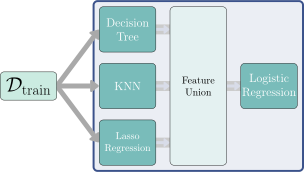
\includegraphics[width=0.7\textwidth,height=\textheight]{chapters/chapter8/Figures/mlr3book_figures-27.png}

}

\caption{\label{fig-pipelines-stacking}Graph that performs Stacking by
fitting three models and using their outputs as features for another
model after combining with \texttt{PipeOpFeatureUnion}.}

\end{figure}

Stacking pipelines depend on the level 0 learners returning predictions
during the \texttt{\$train()} phase. This is possible in
\texttt{mlr3pipelines} with
\href{https://mlr3pipelines.mlr-org.com/reference/mlr_pipeops_learner_cv.html}{\texttt{PipeOpLearnerCV}}\index{\texttt{PipeOpLearnerCV}}.
During training, this operator performs cross-validation and passes the
out-of-sample predictions to the level 1 model. Using cross-validated
predictions is recommended to reduce the risk of overfitting.

We first create the level 0 learners to produce the predictions that
will be used as features. In this example, we use a classification
tree\index{decision tree}, k-nearest
neighbors\index{k-nearest neighbors}
(KNN)\index{KNN|see{k-nearest neighbors}}, and a regularized
GLM\index{generalized linear model}. Each learner is wrapped in
\texttt{po("learner\_cv")} which performs cross-validation on the input
data and then outputs the predictions from the
\href{https://mlr3.mlr-org.com/reference/Learner.html}{\texttt{Learner}}
in a new
\href{https://mlr3.mlr-org.com/reference/Task.html}{\texttt{Task}}
object.

\begin{Shaded}
\begin{Highlighting}[]
\NormalTok{lrn\_rpart }\OtherTok{=} \FunctionTok{lrn}\NormalTok{(}\StringTok{"classif.rpart"}\NormalTok{, }\AttributeTok{predict\_type =} \StringTok{"prob"}\NormalTok{)}
\NormalTok{po\_rpart\_cv }\OtherTok{=} \FunctionTok{po}\NormalTok{(}\StringTok{"learner\_cv"}\NormalTok{, }\AttributeTok{learner =}\NormalTok{ lrn\_rpart,}
  \AttributeTok{resampling.folds =} \DecValTok{2}\NormalTok{, }\AttributeTok{id =} \StringTok{"rpart\_cv"}
\NormalTok{)}

\NormalTok{lrn\_knn }\OtherTok{=} \FunctionTok{lrn}\NormalTok{(}\StringTok{"classif.kknn"}\NormalTok{, }\AttributeTok{predict\_type =} \StringTok{"prob"}\NormalTok{)}
\NormalTok{po\_knn\_cv }\OtherTok{=} \FunctionTok{po}\NormalTok{(}\StringTok{"learner\_cv"}\NormalTok{,}
  \AttributeTok{learner =}\NormalTok{ lrn\_knn,}
  \AttributeTok{resampling.folds =} \DecValTok{2}\NormalTok{, }\AttributeTok{id =} \StringTok{"knn\_cv"}
\NormalTok{)}

\NormalTok{lrn\_glmnet }\OtherTok{=} \FunctionTok{lrn}\NormalTok{(}\StringTok{"classif.glmnet"}\NormalTok{, }\AttributeTok{predict\_type =} \StringTok{"prob"}\NormalTok{)}
\NormalTok{po\_glmnet\_cv }\OtherTok{=} \FunctionTok{po}\NormalTok{(}\StringTok{"learner\_cv"}\NormalTok{,}
  \AttributeTok{learner =}\NormalTok{ lrn\_glmnet,}
  \AttributeTok{resampling.folds =} \DecValTok{2}\NormalTok{, }\AttributeTok{id =} \StringTok{"glmnet\_cv"}
\NormalTok{)}
\end{Highlighting}
\end{Shaded}

These learners are combined using
\href{https://mlr3pipelines.mlr-org.com/reference/gunion.html}{\texttt{gunion()}},
and \texttt{po("featureunion")} is used to merge their predictions. This
is demonstrated in the output of \texttt{\$train()}:

\begin{Shaded}
\begin{Highlighting}[]
\NormalTok{gr\_level\_0 }\OtherTok{=} \FunctionTok{gunion}\NormalTok{(}\FunctionTok{list}\NormalTok{(po\_rpart\_cv, po\_knn\_cv, po\_glmnet\_cv))}
\NormalTok{gr\_combined }\OtherTok{=}\NormalTok{ gr\_level\_0 }\SpecialCharTok{\%\textgreater{}\textgreater{}\%} \FunctionTok{po}\NormalTok{(}\StringTok{"featureunion"}\NormalTok{)}

\NormalTok{gr\_combined}\SpecialCharTok{$}\FunctionTok{train}\NormalTok{(}\FunctionTok{tsk}\NormalTok{(}\StringTok{"sonar"}\NormalTok{))[[}\DecValTok{1}\NormalTok{]]}\SpecialCharTok{$}\FunctionTok{head}\NormalTok{()}
\end{Highlighting}
\end{Shaded}

\begin{verbatim}
   Class rpart_cv.prob.M rpart_cv.prob.R knn_cv.prob.M knn_cv.prob.R
1:     R         0.57895          0.4211        0.3857        0.6143
2:     R         0.88636          0.1136        0.3170        0.6830
3:     R         0.04348          0.9565        0.4396        0.5604
4:     R         0.03030          0.9697        0.4762        0.5238
5:     R         0.04348          0.9565        0.4753        0.5247
6:     R         0.23077          0.7692        0.4020        0.5980
2 variables not shown: [glmnet_cv.prob.M, glmnet_cv.prob.R]
\end{verbatim}

\begin{tcolorbox}[enhanced jigsaw, opacitybacktitle=0.6, rightrule=.15mm, opacityback=0, arc=.35mm, breakable, titlerule=0mm, colframe=quarto-callout-tip-color-frame, coltitle=black, bottomrule=.15mm, toprule=.15mm, colback=white, colbacktitle=quarto-callout-tip-color!10!white, bottomtitle=1mm, toptitle=1mm, title=\textcolor{quarto-callout-tip-color}{\faLightbulb}\hspace{0.5em}{Retaining Features}, leftrule=.75mm, left=2mm]

In this example, the original features were removed as each
\texttt{PipeOp} only returns the predictions made by the respective
learners. To retain the original features, include \texttt{po("nop")} in
the list passed to
\href{https://mlr3pipelines.mlr-org.com/reference/gunion.html}{\texttt{gunion()}}.

\end{tcolorbox}

The resulting task contains the predicted probabilities for both classes
made from each of the level 0 learners. However, as the probabilities
always add up to \(1\), we only need the predictions for one of the
classes (as this is a binary classification task), so we can use
\texttt{po("select")} to only keep predictions for one class (we choose
\texttt{"M"} in this example).

\begin{Shaded}
\begin{Highlighting}[]
\NormalTok{gr\_stack }\OtherTok{=}\NormalTok{ gr\_combined }\SpecialCharTok{\%\textgreater{}\textgreater{}\%}
  \FunctionTok{po}\NormalTok{(}\StringTok{"select"}\NormalTok{, }\AttributeTok{selector =} \FunctionTok{selector\_grep}\NormalTok{(}\StringTok{"}\SpecialCharTok{\textbackslash{}\textbackslash{}}\StringTok{.M$"}\NormalTok{))}
\end{Highlighting}
\end{Shaded}

Finally, we can combine our pipeline with the final model that will take
these predictions as its input. Below we use logistic
regression\index{logistic regression}, which combines the level 0
predictions in a weighted linear sum.

\begin{Shaded}
\begin{Highlighting}[]
\NormalTok{gr\_stack }\OtherTok{=}\NormalTok{ gr\_stack }\SpecialCharTok{\%\textgreater{}\textgreater{}\%} \FunctionTok{po}\NormalTok{(}\StringTok{"learner"}\NormalTok{, }\FunctionTok{lrn}\NormalTok{(}\StringTok{"classif.log\_reg"}\NormalTok{))}
\NormalTok{gr\_stack}\SpecialCharTok{$}\FunctionTok{plot}\NormalTok{(}\AttributeTok{horizontal =} \ConstantTok{TRUE}\NormalTok{)}
\end{Highlighting}
\end{Shaded}

\begin{figure}

{\centering \includegraphics[width=1\textwidth,height=\textheight]{chapters/chapter8/non-sequential_pipelines_and_tuning_files/figure-pdf/fig-pipelines-stackinggraph-1.png}

}

\caption{\label{fig-pipelines-stackinggraph}Constructed stacking Graph
with one input being passed to three weak learners whose predictions are
passed to the logistic regression.}

\end{figure}

As our final model was an interpretable logistic regression, we can
inspect the weights of the level 0 learners by looking at the final
trained model:

\begin{Shaded}
\begin{Highlighting}[]
\NormalTok{glrn\_stack }\OtherTok{=} \FunctionTok{as\_learner}\NormalTok{(gr\_stack)}
\NormalTok{glrn\_stack}\SpecialCharTok{$}\FunctionTok{train}\NormalTok{(}\FunctionTok{tsk}\NormalTok{(}\StringTok{"sonar"}\NormalTok{))}
\NormalTok{glrn\_stack}\SpecialCharTok{$}\FunctionTok{base\_learner}\NormalTok{()}\SpecialCharTok{$}\NormalTok{model}
\end{Highlighting}
\end{Shaded}

\begin{verbatim}

Call:  stats::glm(formula = task$formula(), family = "binomial", data = data, 
    model = FALSE)

Coefficients:
     (Intercept)   rpart_cv.prob.M     knn_cv.prob.M  glmnet_cv.prob.M  
          -3.120            -0.134             4.040             1.804  

Degrees of Freedom: 207 Total (i.e. Null);  204 Residual
Null Deviance:      287 
Residual Deviance: 176  AIC: 184
\end{verbatim}

The model weights suggest that knn influences the predictions the most
with the largest coefficient. To confirm this we can benchmark the
individual models alongside the stacking pipeline.

\begin{Shaded}
\begin{Highlighting}[]
\NormalTok{glrn\_stack}\SpecialCharTok{$}\NormalTok{id }\OtherTok{=} \StringTok{"stacking"}
\NormalTok{design }\OtherTok{=} \FunctionTok{benchmark\_grid}\NormalTok{(}\FunctionTok{tsk}\NormalTok{(}\StringTok{"sonar"}\NormalTok{),}
  \FunctionTok{list}\NormalTok{(lrn\_rpart, lrn\_knn, lrn\_glmnet, glrn\_stack), }\FunctionTok{rsmp}\NormalTok{(}\StringTok{"repeated\_cv"}\NormalTok{))}
\NormalTok{bmr }\OtherTok{=} \FunctionTok{benchmark}\NormalTok{(design)}
\NormalTok{bmr}\SpecialCharTok{$}\FunctionTok{aggregate}\NormalTok{()[, .(learner\_id, classif.ce)]}
\end{Highlighting}
\end{Shaded}

\begin{verbatim}
       learner_id classif.ce
1:  classif.rpart     0.2876
2:   classif.kknn     0.1505
3: classif.glmnet     0.2559
4:       stacking     0.1438
\end{verbatim}

This experiment confirms that of the individual models, the KNN learner
performs the best, however, our stacking pipeline outperforms them all.
Now that we have seen the inner workings of this pipeline, next time you
might want to more efficiently create it using \texttt{ppl("stacking")},
to copy the example above you would run:

\begin{Shaded}
\begin{Highlighting}[]
\FunctionTok{ppl}\NormalTok{(}\StringTok{"stacking"}\NormalTok{,}
  \AttributeTok{base\_learners =} \FunctionTok{lrns}\NormalTok{(}\FunctionTok{c}\NormalTok{(}\StringTok{"classif.rpart"}\NormalTok{, }\StringTok{"classif.kknn"}\NormalTok{,}
    \StringTok{"classif.glmnet"}\NormalTok{)),}
  \AttributeTok{super\_learner =} \FunctionTok{lrn}\NormalTok{(}\StringTok{"classif.log\_reg"}\NormalTok{)}
\NormalTok{)}
\end{Highlighting}
\end{Shaded}

Having covered the building blocks of \texttt{mlr3pipelines} and seen
these in practice, we will now turn to more advanced functionality,
combining pipelines with tuning.

\hypertarget{sec-pipelines-tuning}{%
\section{\texorpdfstring{Tuning\index{tuning}
Graphs}{Tuning Graphs}}\label{sec-pipelines-tuning}}

By wrapping a pipeline inside a
\href{https://mlr3pipelines.mlr-org.com/reference/mlr_learners_graph.html}{\texttt{GraphLearner}},
we can tune it at two levels of complexity using
\href{https://mlr3tuning.mlr-org.com}{\texttt{mlr3tuning}}\index{\texttt{mlr3tuning}}:

\begin{enumerate}
\def\labelenumi{\arabic{enumi}.}
\item
  Tuning of a fixed, usually sequential pipeline, where preprocessing is
  combined with a given learner. This simply means the joint tuning of
  any subset of selected hyperparameters of operations in the pipeline.
  Conceptually and also technically in \texttt{mlr3}, this is not much
  different from tuning a learner that is not part of a pipeline.
\item
  Tuning not only the hyperparameters of a pipeline, whose structure is
  not completely fixed in terms of its included operations, but also
  which concrete
  \href{https://mlr3pipelines.mlr-org.com/reference/PipeOp.html}{\texttt{PipeOp}}s
  should be applied to data. This allows us to select these operations
  (e.g.~which learner to use, which preprocessing to perform) in a
  data-driven manner known as ``Combined Algorithm Selection and
  Hyperparameter
  optimization\index{combined algorithm selection and hyperparameter optimization}''\index{CASH|see{combined algorithm selection and hyperparameter optimization}}
  (Thornton et al. 2013). As we will soon see, we can do this in
  \texttt{mlr3pipelines} by using the powerful branching
  (Section~\ref{sec-pipelines-branch}) and proxy
  (Section~\ref{sec-pipelines-proxy}) meta operators. Through this, we
  can conveniently create our own ``mini AutoML systems'' (Hutter,
  Kotthoff, and Vanschoren 2019) in \texttt{mlr3}, which can even be
  geared for specific tasks.
\end{enumerate}

\hypertarget{sec-pipelines-combined}{%
\subsection{Tuning Graph Hyperparameters}\label{sec-pipelines-combined}}

Let us consider a simple, sequential pipeline using \texttt{po("pca")}
followed by \texttt{lrn("classif.kknn")}:

\begin{Shaded}
\begin{Highlighting}[]
\NormalTok{graph\_learner }\OtherTok{=} \FunctionTok{as\_learner}\NormalTok{(}\FunctionTok{po}\NormalTok{(}\StringTok{"pca"}\NormalTok{) }\SpecialCharTok{\%\textgreater{}\textgreater{}\%} \FunctionTok{lrn}\NormalTok{(}\StringTok{"classif.kknn"}\NormalTok{))}
\end{Highlighting}
\end{Shaded}

The optimal setting of the \texttt{rank.} hyperparameter of our PCA
\href{https://mlr3pipelines.mlr-org.com/reference/PipeOp.html}{\texttt{PipeOp}}
may realistically depend on the value of the \texttt{k} hyperparameter
of the KNN model so jointly tuning them is reasonable. For this, we can
simply use the syntax for tuning \texttt{Learner}s, which was introduced
in Chapter~\ref{sec-optimization}.

\begin{Shaded}
\begin{Highlighting}[]
\NormalTok{lrn\_knn }\OtherTok{=} \FunctionTok{lrn}\NormalTok{(}\StringTok{"classif.kknn"}\NormalTok{, }\AttributeTok{k =} \FunctionTok{to\_tune}\NormalTok{(}\DecValTok{1}\NormalTok{, }\DecValTok{32}\NormalTok{))}
\NormalTok{po\_pca }\OtherTok{=} \FunctionTok{po}\NormalTok{(}\StringTok{"pca"}\NormalTok{, }\AttributeTok{rank. =} \FunctionTok{to\_tune}\NormalTok{(}\DecValTok{2}\NormalTok{, }\DecValTok{20}\NormalTok{))}
\NormalTok{graph\_learner }\OtherTok{=} \FunctionTok{as\_learner}\NormalTok{(po\_pca }\SpecialCharTok{\%\textgreater{}\textgreater{}\%}\NormalTok{ lrn\_knn)}
\NormalTok{graph\_learner}\SpecialCharTok{$}\NormalTok{param\_set}\SpecialCharTok{$}\NormalTok{values}
\end{Highlighting}
\end{Shaded}

\begin{verbatim}
$pca.rank.
Tuning over:
range [2, 20]


$classif.kknn.k
Tuning over:
range [1, 32]
\end{verbatim}

We can see how the pipeline's \texttt{\$param\_set} includes the tune
tokens for all selected hyperparameters, creating a joint search space.
We can compare the tuned and untuned pipeline in a benchmark experiment
with nested resampling by using an \texttt{AutoTuner}:

\begin{Shaded}
\begin{Highlighting}[]
\NormalTok{glrn\_tuned }\OtherTok{=} \FunctionTok{auto\_tuner}\NormalTok{(}\FunctionTok{tnr}\NormalTok{(}\StringTok{"random\_search"}\NormalTok{), graph\_learner,}
  \FunctionTok{rsmp}\NormalTok{(}\StringTok{"holdout"}\NormalTok{), }\AttributeTok{term\_evals =} \DecValTok{10}\NormalTok{)}
\NormalTok{glrn\_untuned }\OtherTok{=} \FunctionTok{po}\NormalTok{(}\StringTok{"pca"}\NormalTok{) }\SpecialCharTok{\%\textgreater{}\textgreater{}\%} \FunctionTok{lrn}\NormalTok{(}\StringTok{"classif.kknn"}\NormalTok{)}
\NormalTok{design }\OtherTok{=} \FunctionTok{benchmark\_grid}\NormalTok{(}\FunctionTok{tsk}\NormalTok{(}\StringTok{"sonar"}\NormalTok{), }\FunctionTok{c}\NormalTok{(glrn\_tuned, glrn\_untuned),}
  \FunctionTok{rsmp}\NormalTok{(}\StringTok{"cv"}\NormalTok{, }\AttributeTok{folds =} \DecValTok{5}\NormalTok{))}
\FunctionTok{benchmark}\NormalTok{(design)}\SpecialCharTok{$}\FunctionTok{aggregate}\NormalTok{()[, .(learner\_id, classif.ce)]}
\end{Highlighting}
\end{Shaded}

\begin{verbatim}
               learner_id classif.ce
1: pca.classif.kknn.tuned     0.2063
2:       pca.classif.kknn     0.2553
\end{verbatim}

Tuning pipelines will usually take longer than tuning individual
learners as training steps are often more complex and the search space
will be larger. Therefore, parallelization is often appropriate
(Section~\ref{sec-parallelization}) and/or more efficient tuning methods
for searching large tuning spaces such as Bayesian
optimization\index{Bayesian optimization}
(Section~\ref{sec-bayesian-optimization}).

\hypertarget{sec-pipelines-branch}{%
\subsection{Tuning Alternative Paths with
po(``branch'')}\label{sec-pipelines-branch}}

In the previous section, we tuned the KKNN and decision
tree\index{decision tree} in the stacking pipeline, as well as tuning
the rank of the PCA. However, we tuned the PCA without first considering
if it was even beneficial at all, in this section we will answer that
question by making use of
\href{https://mlr3pipelines.mlr-org.com/reference/mlr_pipeops_branch.html}{\texttt{PipeOpBranch}}
and
\href{https://mlr3pipelines.mlr-org.com/reference/mlr_pipeops_unbranch.html}{\texttt{PipeOpUnbranch}},
which make it possible to specify multiple alternative paths in a
pipeline. \texttt{po("branch")} creates multiple paths such that data
can only flow through \emph{one} of these as determined by the
\texttt{selection} hyperparameter
(Figure~\ref{fig-pipelines-alternatives}). This concept makes it
possible to use tuning to decide which
\href{https://mlr3pipelines.mlr-org.com/reference/PipeOp.html}{\texttt{PipeOp}}s
and
\href{https://mlr3.mlr-org.com/reference/Learner.html}{\texttt{Learner}}s
to include in the pipeline, while also allowing all options in every
path to be tuned.

\begin{figure}

{\centering 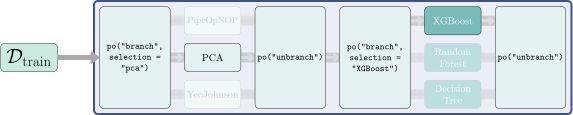
\includegraphics[width=1\textwidth,height=\textheight]{chapters/chapter8/Figures/mlr3book_figures-24.png}

}

\caption{\label{fig-pipelines-branching}Figure demonstrates the
\texttt{po("branch")} and \texttt{po("unbranch")} operators where three
separate branches are created and data only flows through the PCA, which
is specified with the argument to \texttt{selection}.}

\end{figure}

To demonstrate alternative paths we will make use of the MNIST (LeCun et
al. 1998) data, which is useful for demonstrating preprocessing. The
data is loaded from OpenML, which is described in
Section~\ref{sec-openml}, we subset the data to make the example run
faster.

\begin{Shaded}
\begin{Highlighting}[]
\FunctionTok{library}\NormalTok{(mlr3oml)}
\NormalTok{otsk\_mnist }\OtherTok{=} \FunctionTok{otsk}\NormalTok{(}\AttributeTok{id =} \DecValTok{3573}\NormalTok{)}
\NormalTok{tsk\_mnist }\OtherTok{=} \FunctionTok{as\_task}\NormalTok{(otsk\_mnist)}\SpecialCharTok{$}
  \FunctionTok{filter}\NormalTok{(}\FunctionTok{sample}\NormalTok{(}\DecValTok{70000}\NormalTok{, }\DecValTok{1000}\NormalTok{))}\SpecialCharTok{$}
  \FunctionTok{select}\NormalTok{(otsk\_mnist}\SpecialCharTok{$}\NormalTok{feature\_names[}\FunctionTok{sample}\NormalTok{(}\DecValTok{700}\NormalTok{, }\DecValTok{100}\NormalTok{)])}
\end{Highlighting}
\end{Shaded}

\texttt{po("branch")} is initialized either with the number of branches
or with a \texttt{character}-vector indicating the names of the
branches, the latter makes the \texttt{selection} hyperparameter
(discussed below) more readable. Below we create three branches: do
nothing (\texttt{po("nop")}), apply PCA (\texttt{po("pca")}), remove
constant features (\texttt{po("removeconstants")}) then apply the
Yeo-Johnson\index{Yeo-Johnson} transform (\texttt{po("yeojohnson")}). It
is important to use \texttt{po("unbranch")} (with the same arguments as
\texttt{"branch"}) to ensure that the outputs are merged into one result
object.

\begin{Shaded}
\begin{Highlighting}[]
\NormalTok{paths }\OtherTok{=} \FunctionTok{c}\NormalTok{(}\StringTok{"nop"}\NormalTok{, }\StringTok{"pca"}\NormalTok{, }\StringTok{"yeojohnson"}\NormalTok{)}

\NormalTok{graph }\OtherTok{=} \FunctionTok{po}\NormalTok{(}\StringTok{"branch"}\NormalTok{, paths, }\AttributeTok{id =} \StringTok{"brnchPO"}\NormalTok{) }\SpecialCharTok{\%\textgreater{}\textgreater{}\%}
  \FunctionTok{gunion}\NormalTok{(}\FunctionTok{list}\NormalTok{(}
    \FunctionTok{po}\NormalTok{(}\StringTok{"nop"}\NormalTok{),}
    \FunctionTok{po}\NormalTok{(}\StringTok{"pca"}\NormalTok{),}
    \FunctionTok{po}\NormalTok{(}\StringTok{"removeconstants"}\NormalTok{, }\AttributeTok{id =} \StringTok{"rm\_const"}\NormalTok{) }\SpecialCharTok{\%\textgreater{}\textgreater{}\%}
      \FunctionTok{po}\NormalTok{(}\StringTok{"yeojohnson"}\NormalTok{, }\AttributeTok{id =} \StringTok{"YJ"}\NormalTok{)}
\NormalTok{  )) }\SpecialCharTok{\%\textgreater{}\textgreater{}\%} \FunctionTok{po}\NormalTok{(}\StringTok{"unbranch"}\NormalTok{, paths, }\AttributeTok{id =} \StringTok{"unbrnchPO"}\NormalTok{)}

\NormalTok{graph}\SpecialCharTok{$}\FunctionTok{plot}\NormalTok{(}\AttributeTok{horizontal =} \ConstantTok{TRUE}\NormalTok{)}
\end{Highlighting}
\end{Shaded}

\begin{figure}

{\centering \includegraphics[width=1\textwidth,height=\textheight]{chapters/chapter8/non-sequential_pipelines_and_tuning_files/figure-pdf/fig-pipelines-branchone-1.png}

}

\caption{\label{fig-pipelines-branchone}Graph with branching to three
different paths that are split with \texttt{po("branch")} and combined
with \texttt{po("unbranch")}.}

\end{figure}

We can see how the output of this \texttt{Graph} depends on the setting
of the \texttt{branch.selection} hyperparameter:

\begin{Shaded}
\begin{Highlighting}[]
\CommentTok{\# use the "PCA" path}
\NormalTok{graph}\SpecialCharTok{$}\NormalTok{param\_set}\SpecialCharTok{$}\NormalTok{values}\SpecialCharTok{$}\NormalTok{brnchPO.selection }\OtherTok{=} \StringTok{"pca"}
\CommentTok{\# new PCA columns}
\FunctionTok{head}\NormalTok{(graph}\SpecialCharTok{$}\FunctionTok{train}\NormalTok{(tsk\_mnist)[[}\DecValTok{1}\NormalTok{]]}\SpecialCharTok{$}\NormalTok{feature\_names)}
\end{Highlighting}
\end{Shaded}

\begin{verbatim}
[1] "PC1" "PC2" "PC3" "PC4" "PC5" "PC6"
\end{verbatim}

\begin{Shaded}
\begin{Highlighting}[]
\CommentTok{\# use the "No{-}Op" path}
\NormalTok{graph}\SpecialCharTok{$}\NormalTok{param\_set}\SpecialCharTok{$}\NormalTok{values}\SpecialCharTok{$}\NormalTok{brnchPO.selection }\OtherTok{=} \StringTok{"nop"}
\CommentTok{\# same features}
\FunctionTok{head}\NormalTok{(graph}\SpecialCharTok{$}\FunctionTok{train}\NormalTok{(tsk\_mnist)[[}\DecValTok{1}\NormalTok{]]}\SpecialCharTok{$}\NormalTok{feature\_names)}
\end{Highlighting}
\end{Shaded}

\begin{verbatim}
[1] "pixel4"  "pixel10" "pixel11" "pixel14" "pixel34" "pixel39"
\end{verbatim}

\texttt{ppl("branch")} simplifies the above by allowing you to just pass
the different paths to the \texttt{graphs} argument (omitting
``\texttt{rm\_const}'' for simplicity here):

\begin{Shaded}
\begin{Highlighting}[]
\FunctionTok{ppl}\NormalTok{(}\StringTok{"branch"}\NormalTok{, }\AttributeTok{graphs =} \FunctionTok{pos}\NormalTok{(}\FunctionTok{c}\NormalTok{(}\StringTok{"nop"}\NormalTok{, }\StringTok{"pca"}\NormalTok{, }\StringTok{"yeojohnson"}\NormalTok{)))}
\end{Highlighting}
\end{Shaded}

Branching can even be used to tune which of several learners is most
appropriate for a given dataset. We extend our example further and add
the choice between a decision tree and KKNN:

\begin{Shaded}
\begin{Highlighting}[]
\NormalTok{graph\_learner }\OtherTok{=}\NormalTok{ graph }\SpecialCharTok{\%\textgreater{}\textgreater{}\%}
  \FunctionTok{ppl}\NormalTok{(}\StringTok{"branch"}\NormalTok{, }\FunctionTok{lrns}\NormalTok{(}\FunctionTok{c}\NormalTok{(}\StringTok{"classif.rpart"}\NormalTok{, }\StringTok{"classif.kknn"}\NormalTok{)))}
\NormalTok{graph\_learner}\SpecialCharTok{$}\FunctionTok{plot}\NormalTok{(}\AttributeTok{horizontal =} \ConstantTok{TRUE}\NormalTok{)}
\end{Highlighting}
\end{Shaded}

\begin{figure}

{\centering \includegraphics[width=1\textwidth,height=\textheight]{chapters/chapter8/non-sequential_pipelines_and_tuning_files/figure-pdf/fig-pipelines-branchtwo-1.png}

}

\caption{\label{fig-pipelines-branchtwo}Graph with branching to three
different paths that are split with \texttt{po("branch")} and combined
with \texttt{po("unbranch")} then branch and recombine again.}

\end{figure}

Tuning the \texttt{selection} hyperparameters can help determine which
of the possible options work best in combination. We additionally tune
the \texttt{k} hyperparameter of the KNN learner, as it may depend on
the type of preprocessing performed. As this hyperparameter is only
active when the \texttt{"classif.kknn"} path is chosen we will set a
dependency (Section~\ref{sec-optimization-depends}):

\begin{Shaded}
\begin{Highlighting}[]
\NormalTok{graph\_learner }\OtherTok{=} \FunctionTok{as\_learner}\NormalTok{(graph\_learner)}

\NormalTok{graph\_learner}\SpecialCharTok{$}\NormalTok{param\_set}\SpecialCharTok{$}\FunctionTok{set\_values}\NormalTok{(}
  \AttributeTok{brnchPO.selection =} \FunctionTok{to\_tune}\NormalTok{(paths),}
  \AttributeTok{branch.selection =} \FunctionTok{to\_tune}\NormalTok{(}\FunctionTok{c}\NormalTok{(}\StringTok{"classif.rpart"}\NormalTok{, }\StringTok{"classif.kknn"}\NormalTok{)),}
  \AttributeTok{classif.kknn.k =} \FunctionTok{to\_tune}\NormalTok{(}\FunctionTok{p\_int}\NormalTok{(}\DecValTok{1}\NormalTok{, }\DecValTok{32}\NormalTok{,}
    \AttributeTok{depends =}\NormalTok{ branch.selection }\SpecialCharTok{==} \StringTok{"classif.kknn"}\NormalTok{))}
\NormalTok{)}

\NormalTok{instance }\OtherTok{=} \FunctionTok{tune}\NormalTok{(}\FunctionTok{tnr}\NormalTok{(}\StringTok{"grid\_search"}\NormalTok{), tsk\_mnist, graph\_learner,}
  \FunctionTok{rsmp}\NormalTok{(}\StringTok{"repeated\_cv"}\NormalTok{, }\AttributeTok{folds =} \DecValTok{3}\NormalTok{, }\AttributeTok{repeats =} \DecValTok{3}\NormalTok{), }\FunctionTok{msr}\NormalTok{(}\StringTok{"classif.ce"}\NormalTok{))}

\NormalTok{instance}\SpecialCharTok{$}\NormalTok{archive}\SpecialCharTok{$}\NormalTok{data[}\FunctionTok{order}\NormalTok{(classif.ce)[}\DecValTok{1}\SpecialCharTok{:}\DecValTok{5}\NormalTok{],}
\NormalTok{  .(brnchPO.selection, classif.kknn.k, branch.selection, classif.ce)]}
\end{Highlighting}
\end{Shaded}

\begin{verbatim}
   brnchPO.selection classif.kknn.k branch.selection classif.ce
1:        yeojohnson             11     classif.kknn     0.2293
2:        yeojohnson             15     classif.kknn     0.2370
3:        yeojohnson             18     classif.kknn     0.2400
4:        yeojohnson              8     classif.kknn     0.2400
5:        yeojohnson             22     classif.kknn     0.2467
\end{verbatim}

\begin{Shaded}
\begin{Highlighting}[]
\FunctionTok{autoplot}\NormalTok{(instance)}
\end{Highlighting}
\end{Shaded}

\begin{figure}

{\centering \includegraphics[width=1\textwidth,height=\textheight]{chapters/chapter8/non-sequential_pipelines_and_tuning_files/figure-pdf/fig-nonseq-instance-1.pdf}

}

\caption{\label{fig-nonseq-instance}Instance after tuning preprocessing
branch choice (\texttt{brnchPO.selection}), KNN \texttt{k} parameter
(\texttt{classif.kknn.k}), and learning branch choice
(\texttt{branch.selection}). Dots are different hyperparameter
configurations that were tested during tuning, colors separate
hyperparameter configurations.}

\end{figure}

As we can see in the results and Figure~\ref{fig-nonseq-instance}, the
KNN-learner with \texttt{k} set to 11 was selected, which performs best
in combination with the Yeo-Johnson transform.

\hypertarget{sec-pipelines-proxy}{%
\subsection{Tuning with po(``proxy'')}\label{sec-pipelines-proxy}}

\begin{tcolorbox}[enhanced jigsaw, colframe=quarto-callout-note-color-frame, rightrule=.15mm, bottomrule=.15mm, toprule=.15mm, opacityback=0, colback=white, left=2mm, arc=.35mm, breakable, leftrule=.75mm]
\begin{minipage}[t]{5.5mm}
\textcolor{quarto-callout-note-color}{\faInfo}
\end{minipage}%
\begin{minipage}[t]{\textwidth - 5.5mm}

\textbf{This section covers advanced ML or technical
details.}\vspace{2mm}

\end{minipage}%
\end{tcolorbox}

\texttt{po("proxy")} is a meta-operator that performs the operation that
is stored in its \texttt{content} hyperparameter, which could be another
\href{https://mlr3pipelines.mlr-org.com/reference/PipeOp.html}{\texttt{PipeOp}}
or
\href{https://mlr3pipelines.mlr-org.com/reference/Graph.html}{\texttt{Graph}}.
It can therefore be used to tune over and select different
\texttt{PipeOp}s or \texttt{Graph}s that could be passed to this
hyperparameter (Figure~\ref{fig-pipelines-alternatives}).

\begin{figure}

{\centering 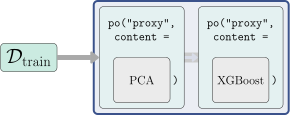
\includegraphics[width=0.7\textwidth,height=\textheight]{chapters/chapter8/Figures/mlr3book_figures-25.png}

}

\caption{\label{fig-pipelines-alternatives}Figure demonstrates the
\texttt{po("proxy")} operator with a \texttt{PipeOp} as its argument.}

\end{figure}

To recreate the example above with \texttt{po("proxy")}, the first step
is to create placeholder
\href{https://mlr3pipelines.mlr-org.com/reference/mlr_pipeops_proxy.html}{\texttt{PipeOpProxy}}
operators to stand in for the operations (i.e., different paths) that
should be tuned.

\begin{Shaded}
\begin{Highlighting}[]
\NormalTok{graph\_learner }\OtherTok{=} \FunctionTok{po}\NormalTok{(}\StringTok{"proxy"}\NormalTok{, }\AttributeTok{id =} \StringTok{"preproc"}\NormalTok{) }\SpecialCharTok{\%\textgreater{}\textgreater{}\%}
  \FunctionTok{po}\NormalTok{(}\StringTok{"proxy"}\NormalTok{, }\AttributeTok{id =} \StringTok{"learner"}\NormalTok{)}
\NormalTok{graph\_learner }\OtherTok{=} \FunctionTok{as\_learner}\NormalTok{(graph\_learner)}
\end{Highlighting}
\end{Shaded}

The tuning space for the \texttt{content} hyperparameters should be a
discrete set of possibilities to be evaluated, passed as a
\href{https://paradox.mlr-org.com/reference/Domain.html}{\texttt{p\_fct}}
(Section~\ref{sec-tune-ps}). For the \texttt{"preproc"} proxy operator
this would simply be the different \texttt{PipeOp}s that we want to
consider:

\begin{Shaded}
\begin{Highlighting}[]
\CommentTok{\# define content for the preprocessing proxy operator}
\NormalTok{preproc.content }\OtherTok{=} \FunctionTok{p\_fct}\NormalTok{(}\FunctionTok{list}\NormalTok{(}
  \AttributeTok{nop =} \FunctionTok{po}\NormalTok{(}\StringTok{"nop"}\NormalTok{),}
  \AttributeTok{pca =} \FunctionTok{po}\NormalTok{(}\StringTok{"pca"}\NormalTok{),}
  \AttributeTok{yeojohnson =} \FunctionTok{po}\NormalTok{(}\StringTok{"removeconstants"}\NormalTok{) }\SpecialCharTok{\%\textgreater{}\textgreater{}\%} \FunctionTok{po}\NormalTok{(}\StringTok{"yeojohnson"}\NormalTok{)}
\NormalTok{))}
\end{Highlighting}
\end{Shaded}

For the \texttt{"learner"} proxy, this is more complicated as the
selection of the learner depends on more than one search space
component: The choice of the learner itself
(\texttt{lrn("classif.rpart")} or \texttt{lrn("classif.kknn")}) and the
tuned \texttt{k} hyperparameter of the KNN learner. To enable this we
pass a transformation to \texttt{.extra\_trafo}
(Section~\ref{sec-tune-trafo}). Note that inside this transformation we
clone \texttt{learner.content}, otherwise, we would end up modifying the
original
\href{https://mlr3.mlr-org.com/reference/Learner.html}{\texttt{Learner}}
object inside the search space by reference (Section~\ref{sec-r6}).

\begin{Shaded}
\begin{Highlighting}[]
\CommentTok{\# define content for the learner proxy operator}
\NormalTok{learner.content }\OtherTok{=} \FunctionTok{p\_fct}\NormalTok{(}\FunctionTok{list}\NormalTok{(}
    \AttributeTok{classif.rpart =} \FunctionTok{lrn}\NormalTok{(}\StringTok{"classif.rpart"}\NormalTok{),}
    \AttributeTok{classif.kknn =} \FunctionTok{lrn}\NormalTok{(}\StringTok{"classif.kknn"}\NormalTok{)}
\NormalTok{))}

\CommentTok{\# define transformation to set the content values}
\NormalTok{trafo }\OtherTok{=} \ControlFlowTok{function}\NormalTok{(x, param\_set) \{}
    \ControlFlowTok{if}\NormalTok{ (}\SpecialCharTok{!}\FunctionTok{is.null}\NormalTok{(x}\SpecialCharTok{$}\NormalTok{classif.kknn.k)) \{}
\NormalTok{      x}\SpecialCharTok{$}\NormalTok{learner.content }\OtherTok{=}\NormalTok{ x}\SpecialCharTok{$}\NormalTok{learner.content}\SpecialCharTok{$}\FunctionTok{clone}\NormalTok{(}\AttributeTok{deep =} \ConstantTok{TRUE}\NormalTok{)}
\NormalTok{      x}\SpecialCharTok{$}\NormalTok{learner.content}\SpecialCharTok{$}\NormalTok{param\_set}\SpecialCharTok{$}\NormalTok{values}\SpecialCharTok{$}\NormalTok{k }\OtherTok{=}\NormalTok{ x}\SpecialCharTok{$}\NormalTok{classif.kknn.k}
\NormalTok{      x}\SpecialCharTok{$}\NormalTok{classif.kknn.k }\OtherTok{=} \ConstantTok{NULL}
\NormalTok{    \}}
\NormalTok{    x}
\NormalTok{\}}
\end{Highlighting}
\end{Shaded}

We can now put this all together, add the KNN tuning, and run the
experiment.

\begin{Shaded}
\begin{Highlighting}[]
\NormalTok{search\_space }\OtherTok{=} \FunctionTok{ps}\NormalTok{(}
  \AttributeTok{preproc.content =}\NormalTok{ preproc.content,}
  \AttributeTok{learner.content =}\NormalTok{ learner.content,}
  \CommentTok{\# tune KKNN parameter as normal}
  \AttributeTok{classif.kknn.k =} \FunctionTok{p\_int}\NormalTok{(}\DecValTok{1}\NormalTok{, }\DecValTok{32}\NormalTok{,}
    \AttributeTok{depends =}\NormalTok{ learner.content }\SpecialCharTok{==} \StringTok{"classif.kknn"}\NormalTok{),}
  \AttributeTok{.extra\_trafo =}\NormalTok{ trafo}
\NormalTok{)}

\NormalTok{instance }\OtherTok{=} \FunctionTok{tune}\NormalTok{(}\FunctionTok{tnr}\NormalTok{(}\StringTok{"grid\_search"}\NormalTok{), tsk\_mnist, graph\_learner,}
  \FunctionTok{rsmp}\NormalTok{(}\StringTok{"repeated\_cv"}\NormalTok{, }\AttributeTok{folds =} \DecValTok{3}\NormalTok{, }\AttributeTok{repeats =} \DecValTok{3}\NormalTok{), }\FunctionTok{msr}\NormalTok{(}\StringTok{"classif.ce"}\NormalTok{),}
  \AttributeTok{search\_space =}\NormalTok{ search\_space)}

\FunctionTok{as.data.table}\NormalTok{(instance}\SpecialCharTok{$}\NormalTok{result)[,}
\NormalTok{  .(preproc.content,}
    \AttributeTok{classif.kknn.k =}\NormalTok{ x\_domain[[}\DecValTok{1}\NormalTok{]]}\SpecialCharTok{$}\NormalTok{learner.content}\SpecialCharTok{$}\NormalTok{param\_set}\SpecialCharTok{$}\NormalTok{values}\SpecialCharTok{$}\NormalTok{k,}
\NormalTok{    learner.content, classif.ce)}
\NormalTok{]}
\end{Highlighting}
\end{Shaded}

\begin{verbatim}
   preproc.content classif.kknn.k learner.content classif.ce
1:      yeojohnson             11    classif.kknn       0.23
\end{verbatim}

Once again, the best configuration is a KNN learner with the Yeo-Johnson
transform. In practice \texttt{po("proxy")} offers complete flexibility
and may be more useful for more complicated use cases, whereas
\texttt{ppl("branch")} is more efficient in more straightforward
scenarios.

\hypertarget{sec-hyperband-example-svm}{%
\subsection{Hyperband with
Subsampling}\label{sec-hyperband-example-svm}}

\begin{tcolorbox}[enhanced jigsaw, colframe=quarto-callout-note-color-frame, rightrule=.15mm, bottomrule=.15mm, toprule=.15mm, opacityback=0, colback=white, left=2mm, arc=.35mm, breakable, leftrule=.75mm]
\begin{minipage}[t]{5.5mm}
\textcolor{quarto-callout-note-color}{\faInfo}
\end{minipage}%
\begin{minipage}[t]{\textwidth - 5.5mm}

\textbf{This section covers advanced ML or technical
details.}\vspace{2mm}

\end{minipage}%
\end{tcolorbox}

In Section~\ref{sec-hyperband} we learned about the
Hyperband\index{hyperband} tuner and how it can make use of fidelity
parameters\index{fidelity parameters} to efficiently tune learners. Now
that you have learned about pipelines and how to tune them, in this
short section we will briefly return to Hyperband to showcase how we can
put together everything we have learned in this chapter to allow
Hyperband to be used with any \texttt{Learner}.

We previously saw how some learners have hyperparameters that can act
naturally as fidelity parameters, such as the number of trees in a
random forest. However, using pipelines, we can now create a fidelity
parameter for any model using \texttt{po("subsample")}. The
\texttt{frac} parameter of \texttt{po("subsample")} controls the amount
of data fed into the subsequent \texttt{Learner}. In general, feeding
less data to a \texttt{Learner} results in quicker model training but
poorer quality predictions compared to when more training data is
supplied. Resampling with less data will still give us some information
about the relative performance of different model configurations, thus
making the fraction of data to subsample the perfect candidate for a
fidelity parameter.

In this example, we will optimize the SVM\index{support vector machine}
hyperparameters, \texttt{cost} and \texttt{gamma}, on
\texttt{tsk("sonar")}:

\begin{Shaded}
\begin{Highlighting}[]
\FunctionTok{library}\NormalTok{(mlr3tuning)}

\NormalTok{learner }\OtherTok{=} \FunctionTok{lrn}\NormalTok{(}\StringTok{"classif.svm"}\NormalTok{, }\AttributeTok{id =} \StringTok{"svm"}\NormalTok{, }\AttributeTok{type =} \StringTok{"C{-}classification"}\NormalTok{,}
  \AttributeTok{kernel =} \StringTok{"radial"}\NormalTok{, }\AttributeTok{cost  =} \FunctionTok{to\_tune}\NormalTok{(}\FloatTok{1e{-}5}\NormalTok{, }\FloatTok{1e5}\NormalTok{, }\AttributeTok{logscale =} \ConstantTok{TRUE}\NormalTok{),}
  \AttributeTok{gamma =} \FunctionTok{to\_tune}\NormalTok{(}\FloatTok{1e{-}5}\NormalTok{, }\FloatTok{1e5}\NormalTok{, }\AttributeTok{logscale =} \ConstantTok{TRUE}\NormalTok{))}
\end{Highlighting}
\end{Shaded}

We then construct \texttt{po("subsample")} and specify that we want to
use the \texttt{frac} parameter between \([3^{-3}, 1]\) as our fidelity
parameter and set the \texttt{"budget"} tag to pass this information to
Hyperband. We add this to our SVM and create a
\href{https://mlr3pipelines.mlr-org.com/reference/mlr_learners_graph.html}{\texttt{GraphLearner}}.

\begin{Shaded}
\begin{Highlighting}[]
\NormalTok{graph\_learner }\OtherTok{=} \FunctionTok{as\_learner}\NormalTok{(}
  \FunctionTok{po}\NormalTok{(}\StringTok{"subsample"}\NormalTok{, }\AttributeTok{frac =} \FunctionTok{to\_tune}\NormalTok{(}\FunctionTok{p\_dbl}\NormalTok{(}\DecValTok{3}\SpecialCharTok{\^{}{-}}\DecValTok{3}\NormalTok{, }\DecValTok{1}\NormalTok{, }\AttributeTok{tags =} \StringTok{"budget"}\NormalTok{))) }\SpecialCharTok{\%\textgreater{}\textgreater{}\%}
\NormalTok{  learner}
\NormalTok{)}
\end{Highlighting}
\end{Shaded}

As good practice, we encapsulate our learner and add a fallback to
prevent fatal errors (Section~\ref{sec-tuning-errors}).

\begin{Shaded}
\begin{Highlighting}[]
\NormalTok{graph\_learner}\SpecialCharTok{$}\NormalTok{encapsulate }\OtherTok{=} \FunctionTok{c}\NormalTok{(}\AttributeTok{train =} \StringTok{"evaluate"}\NormalTok{, }\AttributeTok{predict =} \StringTok{"evaluate"}\NormalTok{)}
\NormalTok{graph\_learner}\SpecialCharTok{$}\NormalTok{timeout }\OtherTok{=} \FunctionTok{c}\NormalTok{(}\AttributeTok{train =} \DecValTok{30}\NormalTok{, }\AttributeTok{predict =} \DecValTok{30}\NormalTok{)}
\NormalTok{graph\_learner}\SpecialCharTok{$}\NormalTok{fallback }\OtherTok{=} \FunctionTok{lrn}\NormalTok{(}\StringTok{"classif.featureless"}\NormalTok{)}
\end{Highlighting}
\end{Shaded}

Now we can tune our SVM by tuning our \texttt{GraphLearner} as normal,
below we set \texttt{eta\ =\ 3} for Hyperband.

\begin{Shaded}
\begin{Highlighting}[]
\NormalTok{instance }\OtherTok{=} \FunctionTok{tune}\NormalTok{(}\FunctionTok{tnr}\NormalTok{(}\StringTok{"hyperband"}\NormalTok{, }\AttributeTok{eta =} \DecValTok{3}\NormalTok{), }\FunctionTok{tsk}\NormalTok{(}\StringTok{"sonar"}\NormalTok{), graph\_learner,}
  \FunctionTok{rsmp}\NormalTok{(}\StringTok{"cv"}\NormalTok{, }\AttributeTok{folds =} \DecValTok{3}\NormalTok{), }\FunctionTok{msr}\NormalTok{(}\StringTok{"classif.ce"}\NormalTok{))}

\NormalTok{instance}\SpecialCharTok{$}\NormalTok{result\_x\_domain}
\end{Highlighting}
\end{Shaded}

\begin{verbatim}
$subsample.frac
[1] 1

$svm.cost
[1] 5126

$svm.gamma
[1] 0.03179
\end{verbatim}

\hypertarget{sec-pipelines-featsel}{%
\subsection{Feature Selection with Filter
Pipelines}\label{sec-pipelines-featsel}}

\begin{tcolorbox}[enhanced jigsaw, colframe=quarto-callout-note-color-frame, rightrule=.15mm, bottomrule=.15mm, toprule=.15mm, opacityback=0, colback=white, left=2mm, arc=.35mm, breakable, leftrule=.75mm]
\begin{minipage}[t]{5.5mm}
\textcolor{quarto-callout-note-color}{\faInfo}
\end{minipage}%
\begin{minipage}[t]{\textwidth - 5.5mm}

\textbf{This section covers advanced ML or technical
details.}\vspace{2mm}

\end{minipage}%
\end{tcolorbox}

In Section~\ref{sec-fs-filter-based} we learnt about filter-based
feature selection\index{feature selection} and how we can manually run a
filter and then extract the selected features, often using an arbitrary
choice of thresholds that were not tuned. Now that we have covered
pipelines and tuning, we will briefly return to feature selection to
demonstrate how to automate filter-based feature selection by making use
of \texttt{po("filter")}. \texttt{po("filter")} includes the
\texttt{filter} construction argument, which takes a
\href{https://www.rdocumentation.org/packages/base/topics/funprog}{\texttt{Filter}}
object to be used as the filter method as well as a choice of parameters
for different methods of selecting features:

\begin{itemize}
\tightlist
\item
  \texttt{filter.nfeat} -- Number of features to select
\item
  \texttt{filter.frac} -- Fraction of features to select
\item
  \texttt{filter.cutoff} -- Minimum value of filter such that features
  with filter values greater than or equal to the cutoff are kept
\item
  \texttt{filter.permuted} -- Random permutation of features added to
  task before applying the filter and all features before the
  \texttt{permuted}-th permuted features are kept
\end{itemize}

Below we use the information gain filter and select the top three
features:

\begin{Shaded}
\begin{Highlighting}[]
\FunctionTok{library}\NormalTok{(mlr3filters)}
\FunctionTok{library}\NormalTok{(mlr3fselect)}

\NormalTok{task\_pen }\OtherTok{=} \FunctionTok{tsk}\NormalTok{(}\StringTok{"penguins"}\NormalTok{)}

\CommentTok{\# combine filter (keep top 3 features) with learner}
\NormalTok{po\_flt }\OtherTok{=} \FunctionTok{po}\NormalTok{(}\StringTok{"filter"}\NormalTok{, }\AttributeTok{filter =} \FunctionTok{flt}\NormalTok{(}\StringTok{"information\_gain"}\NormalTok{), }\AttributeTok{filter.nfeat =} \DecValTok{3}\NormalTok{)}
\NormalTok{graph }\OtherTok{=}\NormalTok{ po\_flt }\SpecialCharTok{\%\textgreater{}\textgreater{}\%} \FunctionTok{po}\NormalTok{(}\StringTok{"learner"}\NormalTok{, }\FunctionTok{lrn}\NormalTok{(}\StringTok{"classif.rpart"}\NormalTok{))}

\FunctionTok{po}\NormalTok{(}\StringTok{"filter"}\NormalTok{, }\AttributeTok{filter =} \FunctionTok{flt}\NormalTok{(}\StringTok{"information\_gain"}\NormalTok{), }\AttributeTok{filter.nfeat =} \DecValTok{3}\NormalTok{)}\SpecialCharTok{$}
  \FunctionTok{train}\NormalTok{(}\FunctionTok{list}\NormalTok{(task\_pen))[[}\DecValTok{1}\NormalTok{]]}\SpecialCharTok{$}\NormalTok{feature\_names}
\end{Highlighting}
\end{Shaded}

\begin{verbatim}
[1] "bill_depth"     "bill_length"    "flipper_length"
\end{verbatim}

Choosing \texttt{3} as the cutoff was fairly arbitrary but by tuning a
graph we can optimize this cutoff:

\begin{Shaded}
\begin{Highlighting}[]
\CommentTok{\# tune between 1 and total number of features}
\NormalTok{po\_filter }\OtherTok{=} \FunctionTok{po}\NormalTok{(}\StringTok{"filter"}\NormalTok{, }\AttributeTok{filter =} \FunctionTok{flt}\NormalTok{(}\StringTok{"information\_gain"}\NormalTok{),}
  \AttributeTok{filter.nfeat =} \FunctionTok{to\_tune}\NormalTok{(}\DecValTok{1}\NormalTok{, task\_pen}\SpecialCharTok{$}\NormalTok{ncol))}

\NormalTok{graph }\OtherTok{=} \FunctionTok{as\_learner}\NormalTok{(po\_filter }\SpecialCharTok{\%\textgreater{}\textgreater{}\%} \FunctionTok{po}\NormalTok{(}\StringTok{"learner"}\NormalTok{, }\FunctionTok{lrn}\NormalTok{(}\StringTok{"classif.rpart"}\NormalTok{)))}

\NormalTok{instance }\OtherTok{=} \FunctionTok{tune}\NormalTok{(}\FunctionTok{tnr}\NormalTok{(}\StringTok{"random\_search"}\NormalTok{), task\_pen, graph,}
  \FunctionTok{rsmp}\NormalTok{(}\StringTok{"cv"}\NormalTok{, }\AttributeTok{folds =} \DecValTok{3}\NormalTok{), }\AttributeTok{term\_evals =} \DecValTok{10}\NormalTok{)}
\NormalTok{instance}\SpecialCharTok{$}\NormalTok{result}
\end{Highlighting}
\end{Shaded}

\begin{verbatim}
   information_gain.filter.nfeat learner_param_vals  x_domain classif.ce
1:                             5          <list[2]> <list[1]>    0.06972
\end{verbatim}

In this example, \texttt{5} is the optimal number of features. It can be
especially useful in feature selection to visualize the tuning results
as there may be cases where the optimal result is only marginally better
than a result with less features (which would lead to a model that is
quicker to train and possibly easier to interpret).

\begin{Shaded}
\begin{Highlighting}[]
\FunctionTok{autoplot}\NormalTok{(instance)}
\end{Highlighting}
\end{Shaded}

\begin{figure}[H]

{\centering \includegraphics[width=1\textwidth,height=\textheight]{chapters/chapter8/non-sequential_pipelines_and_tuning_files/figure-pdf/fig-tunefilter-1.pdf}

}

\caption{\label{fig-tunefilter}Model performance with different numbers
of features, selected by an information gain filter.}

\end{figure}

Now we can see that four variables may be equally as good in this case
so we could consider going forward by selecting four features and not
six as suggested by \texttt{instance\$result}.

\hypertarget{conclusion-6}{%
\section{Conclusion}\label{conclusion-6}}

In this chapter, we built on what we learned in
Chapter~\ref{sec-pipelines} to develop complex non-sequential
\texttt{Graph}s. We saw how to build our own graphs, as well as how to
make use of \texttt{ppl()} to load \texttt{Graph}s that are available in
\href{https://mlr3pipelines.mlr-org.com}{\texttt{mlr3pipelines}}\index{\texttt{mlr3pipelines}}.
We then looked at different ways to tune pipelines, including joint
tuning of hyperparameters and tuning the selection of \texttt{PipeOp}s
in a \texttt{Graph}, enabling the construction of simple, custom AutoML
systems. In Chapter~\ref{sec-preprocessing} we will study in more detail
how to use pipelines for data preprocessing.

\hypertarget{tbl-api-pipelines-nonseq}{}
\begin{longtable}[]{@{}
  >{\raggedright\arraybackslash}p{(\columnwidth - 4\tabcolsep) * \real{0.3333}}
  >{\raggedright\arraybackslash}p{(\columnwidth - 4\tabcolsep) * \real{0.3333}}
  >{\raggedright\arraybackslash}p{(\columnwidth - 4\tabcolsep) * \real{0.3333}}@{}}
\caption{\label{tbl-api-pipelines-nonseq}Important classes and functions
covered in this chapter with underlying class (if applicable), class
constructor or function, and important class fields and methods (if
applicable).}\tabularnewline
\toprule\noalign{}
\begin{minipage}[b]{\linewidth}\raggedright
Class
\end{minipage} & \begin{minipage}[b]{\linewidth}\raggedright
Constructor/Function
\end{minipage} & \begin{minipage}[b]{\linewidth}\raggedright
Fields/Methods
\end{minipage} \\
\midrule\noalign{}
\endfirsthead
\toprule\noalign{}
\begin{minipage}[b]{\linewidth}\raggedright
Class
\end{minipage} & \begin{minipage}[b]{\linewidth}\raggedright
Constructor/Function
\end{minipage} & \begin{minipage}[b]{\linewidth}\raggedright
Fields/Methods
\end{minipage} \\
\midrule\noalign{}
\endhead
\bottomrule\noalign{}
\endlastfoot
\href{https://mlr3pipelines.mlr-org.com/reference/Graph.html}{\texttt{Graph}}
&
\href{https://mlr3pipelines.mlr-org.com/reference/ppl.html}{\texttt{ppl()}}
& \texttt{\$train()}; \texttt{\$predict()} \\
\href{https://mlr3pipelines.mlr-org.com/reference/Selector.html}{\texttt{Selector}}
&
\href{https://mlr3pipelines.mlr-org.com/reference/Selector.html}{\texttt{selector\_grep()}};
\href{https://mlr3pipelines.mlr-org.com/reference/Selector.html}{\texttt{selector\_type()}};
\href{https://mlr3pipelines.mlr-org.com/reference/Selector.html}{\texttt{selector\_invert()}}
& - \\
\href{https://mlr3pipelines.mlr-org.com/reference/mlr_pipeops_branch.html}{\texttt{PipeOpBranch}};
\href{https://mlr3pipelines.mlr-org.com/reference/mlr_pipeops_unbranch.html}{\texttt{PipeOpUnbranch}}
& \texttt{po("branch")}; \texttt{po("unbranch")} & - \\
\href{https://mlr3pipelines.mlr-org.com/reference/mlr_pipeops_proxy.html}{\texttt{PipeOpProxy}}
& \texttt{po("proxy")} & - \\
\end{longtable}

\hypertarget{exercises-6}{%
\section{Exercises}\label{exercises-6}}

\begin{enumerate}
\def\labelenumi{\arabic{enumi}.}
\tightlist
\item
  Create a graph that replaces all numeric columns that do not contain
  missing values with their PCA transform. Solve this in two ways, using
  \texttt{affect\_columns} in a sequential graph, and using
  \texttt{po("select")} in a non-sequential graph. Train the graph on
  \texttt{tsk("pima")} to check your result. Hint: You may find
  \texttt{selector\_missing()} useful.
\item
  The \texttt{po("select")} in Section~\ref{sec-pipelines-stack} is
  necessary to remove redundant predictions (recall this is a binary
  classification task so we do not require predictions of both classes).
  However, if this was a multiclass classification task, then using
  \texttt{selector\_grep()} would need to be called with a pattern for
  \emph{all} prediction columns that should be \emph{kept}, which would
  be inefficient. Instead it would be more appropriate to provide a
  pattern for the single class to remove. How would you do this using
  the \texttt{Selector} functions provided by \texttt{mlr3pipelines}?
  Implement this and train the modified stacking pipeline on
  \texttt{tsk("wine")}, using \texttt{lrn("classif.multinom")} as the
  level 1 learner.
\item
  How would you solve the previous exercise without explicitly naming
  the class you want to exclude, so that your graph works for any
  classification task? Hint: look at the \texttt{selector\_subsample} in
  Section~\ref{sec-pipelines-bagging}.
\item
  (*) Create your own ``minimal AutoML system'' by combining pipelines,
  branching and tuning. It should allow automatic preprocessing and the
  automatic selection of a well-performing learning algorithm. Both your
  \texttt{PipeOp}s and models should be tuned. Your system should
  feature options for two preprocessing steps (imputation and factor
  encoding) and at least three learning algorithms to choose from. You
  can optimize this via random search, or try to use a more advanced
  tuning algorithm. Test it on at least three different data sets and
  compare its performance against an untuned random forest via nested
  resampling.
\end{enumerate}